\documentclass[a4paper,11pt]{report}
 
 \usepackage[left=3cm, right=3cm, top=3cm, bottom=3cm]{geometry}
\usepackage{graphicx}
\usepackage{listings}
\usepackage{titlesec}
\usepackage{fancyhdr}
\usepackage{epstopdf}
\usepackage{float}
\usepackage{amsmath}
\usepackage{setspace}
\usepackage{eufrak}
\usepackage{url}

\usepackage{courier}
 \newcommand{\textform}[1]{\fontsize{14}{20}\selectfont{#1}}
\pagestyle{fancy}
\fancyhf{}
\fancyhead[R]{\thepage}
\renewcommand{\chaptermark}[1]{\markboth{#1}{}}
\renewcommand{\headrulewidth}{1pt}
\renewcommand{\footrulewidth}{1pt}

\lhead{\footnotesize{EYEPHONE}}
\rhead{}
\lfoot{\footnotesize{Department of Computer Science \& Engg.}}
\cfoot{}
\rfoot{\thepage}

\titleformat{\chapter}[display]
{\normalfont\Large\bfseries\centering}{\chaptertitlename\
\thechapter}{20pt}{\Large}


%\title{\textbf{A seminar report on\\TRUSTWORTHINESS MANAGEMENT IN THE SOCIAL INTERNET OF THINGS} 
%}
%\author{\textbf{Deena Jose}}

\begin{document}

\thispagestyle{empty}
  \begin{center}
      \fontsize{22}{25}\selectfont{\textbf{GOVERNMENT POLYTECHNIC COLLEGE PERUMBAVOOR}}\\[.1cm]
            \fontsize{15}{25}\selectfont{\textbf{Koovappady P.O Ernakulam-683 544 Kerala
    }}\\[1.2cm]
\begin{figure}[h]
	\centering
	\hspace{21pt}
	
\includegraphics[width=.50\linewidth]{logo.png}
	\label{fig:logo.png}
\end{figure}

\fontsize{14}{25}\selectfont{\textbf{Semester - VI}}\\
\fontsize{14}{25}\selectfont{\textbf{Computer Engineering 2022-23}}\\[1.2cm]

\fontsize{14}{25}\selectfont{\textbf{A SEMINAR REPORT}}\\[.1cm]
    \fontsize{14}{25}\selectfont{on}\\
    \fontsize{20}{25}\selectfont{\textbf{EYEPHONE}}\\[1.2cm]
    \end{center}
    \begin{center}
    \fontsize{12}{25}\selectfont{\textbf{Submitted by}}\\[.2cm]
    \fontsize{14}{25}\selectfont \bfseries{AJITH M VIJAYAN}\\[.1cm]
    \fontsize{12}{25}\selectfont{\textbf{20132973}}\\[.2cm]
%\vfill
 \end{center}

\fontsize{12pt}{20}\selectfont
\thispagestyle{empty}


\newpage
  \thispagestyle{empty}

    \begin{center}
      \fontsize{14}{20}\selectfont \textbf{GOVERNMENT POLYTECHNIC COLLEGE PERUMBAVOOR}\\
     
    \fontsize{14}{20}\selectfont \textbf{
DEPARTMENT OF COMPUTER ENGINEERING}\\[1.5cm]
\begin{figure}[h]
\centering
	\hspace{.5cm}

\includegraphics[width=0.3\linewidth]{logo.png}
	\label{fig:logo.png}
\end{figure}

     
      \textbf{CERTIFICATE}
    \end{center}
    \vspace{.5cm}
    \textform{This is to certify that the seminar report entitled \textbf{Eyephone} submitted by \textbf{Ajith M Vijayan}. The seminar report is approved for submission requirement for 6009 -Project and Seminar in  $6^{th}$ semester Computer Engineering at Govt.Polytechnic College,Perumbavoor.}\\[0.15cm]


\begin{minipage}{.31\textwidth}
    \begin{flushleft}
        \begin{center}
            \fontsize{12}{25}\selectfont{\textbf{Head of Section}}\\[1.5cm]
        \end{center}
    \end{flushleft}
\end{minipage}
\hfill
\begin{minipage}{0.40\textwidth}
    \begin{flushright}
        \begin{center}
            \fontsize{12}{25}\selectfont{\textbf{Lecturer in Charge}}\\[1.5cm]
        \end{center}
    \end{flushright}
\end{minipage}



\vspace{1cm}
\begin{flushleft}
  \fontsize{12}{20}\selectfont \textbf{Date  :}\\
  \fontsize{12}{20}\selectfont \textbf{Place :}
\end{flushleft}
\vspace{1cm}
\begin{minipage}{.4\textwidth}
    \begin{flushleft}
    \begin{center}
    
    \fontsize{14}{25}\selectfont \bfseries{Internal Examiner}\\[.1cm]
    
%\vfill
 \end{center}
    \end{flushleft}
      \end{minipage}
\begin{minipage}{0.8\textwidth}
\begin{flushright}
\begin{center}
 
%\vfill
\fontsize{14}{25}\selectfont \bfseries{External Examiner}\\[.1cm]

\end{center}
\end{flushright}
\end{minipage}
\newpage
\fontsize{12pt}{20}\selectfont
\thispagestyle{empty}
  \renewcommand\abstractname{\textform{\textbf{ACKNOWLEDGMENT}}}
    \begin{abstract}
      \vspace{2.5cm}
 I would like to express my sincere gratitude to all those who have contributed to the successful completion of my seminar on synchronous chips. This opportunity has allowed me to delve into a fascinating field of study and expand my knowledge in computer engineering.

First and foremost, I extend my heartfelt appreciation to Dr. Aiju Thomas, the Principal of Government Polytechnic College Perumbavoor. I am grateful for his constant support, guidance, and encouragement throughout my academic journey. His visionary leadership and commitment to excellence have created an environment conducive to learning and exploration.

I am indebted to Mr. Biju Peter, the Head of the Department of Computer Engineering, for his invaluable guidance and mentorship. His expertise, patience, and enthusiasm have been instrumental in shaping my understanding of the subject and honing my research skills. I am thankful for his unwavering support and valuable insights that have enriched my seminar.

I would also like to acknowledge the faculty members of the Computer Engineering Department for their constant support and encouragement throughout my academic journey. Their expertise and passion for teaching have played a significant role in shaping my intellectual growth.

I would like to express my gratitude to my classmates and friends for their support and encouragement. Their presence and collaboration have made the learning experience enjoyable and memorable.
       
    \end{abstract}
 


\thispagestyle{empty}
  \renewcommand\abstractname{\textform{\textbf{ABSTRACT}}}
    \begin{abstract}
      \vspace{1.0cm}

 \paragraph{ }
The Eyephone is a revolutionary smartphone that has transformed the way we interact with technology. This abstract provides an overview of the key aspects and impact of Eyephone in the realm of mobile communication. 

The Eyephone combines cutting-edge hardware and software innovations to deliver a seamless user experience. With its sleek design, high-resolution display, and advanced camera capabilities, Eyephone offers a range of features that cater to the diverse needs of modern smartphone users. 

One of the standout features of Eyephone is its intuitive interface, which is designed to enhance user interaction and accessibility. The user-centered design principles behind Eyephone enable effortless navigation, multi-touch gestures, and voice recognition, empowering users to effortlessly access information, communicate, and engage with a wide range of applications and services.

Beyond its technical prowess, Eyephone has had a profound impact on the smartphone industry and the way we live our lives. It has sparked a wave of innovation and competition, setting new standards for mobile devices. Eyephone's influence can be seen in various aspects, including design trends, app development, and user behavior.

In conclusion, the Eyephone has redefined the smartphone landscape, offering a combination of powerful features, intuitive interface, and seamless user experience. Its impact extends beyond technology, influencing the way we communicate, work, and engage with the digital world. As Eyephone continues to evolve, it is poised to shape the future of mobile technology, driving innovation and transforming the way we connect with the world around us.
\end{abstract}

  \tableofcontents
\thispagestyle{empty}

\chapter{Introduction}

\paragraph{}
The Eyephone is a revolutionary smartphone that has transformed the way we communicate, connect, and experience the digital world. Developed by a leading technology company, the Eyephone has quickly gained global recognition for its cutting-edge design, advanced features, and unparalleled user experience.

With its sleek and elegant design, the Eyephone sets new standards in smartphone aesthetics. Its slim profile, premium materials, and seamless integration of hardware and software make it a true masterpiece of craftsmanship. The Eyephone not only looks visually stunning but also feels comfortable and ergonomic in the hand, providing a delightful tactile experience to its users.

Beyond its captivating design, the Eyephone boasts an array of innovative features and technologies that redefine the boundaries of smartphone capabilities. From its high-resolution display and powerful processor to its advanced camera system and intelligent virtual assistant, the Eyephone offers a comprehensive suite of tools and functionalities that empower users to accomplish tasks, capture memories, and explore endless possibilities.

Furthermore, the Eyephone introduces a seamless and intuitive user interface, ensuring effortless navigation and interaction. Its operating system provides a rich ecosystem of applications and services, catering to diverse interests and needs. Whether it's staying connected with loved ones, managing productivity, or indulging in multimedia entertainment, the Eyephone offers a versatile platform that enhances every aspect of our digital lives.

In this report, we delve into the various aspects of the Eyephone, exploring its design philosophy, technical specifications, and the impact it has made on the mobile industry. We will also examine the implications of Eyephone's features and innovations on user experience, productivity, and societal dynamics.
  
\chapter{Background and History}
The Eyephone, a groundbreaking smartphone, has emerged as a result of the relentless pursuit of innovation and technological advancement in the mobile industry. Developed by a renowned technology company, the Eyephone has revolutionized the way we communicate, access information, and interact with the digital world.

The origins of the Eyephone can be traced back to the early 2000s when mobile phones were primarily used for voice calls and basic messaging. As technology advanced and consumer demands evolved, there was a growing need for a device that could combine multiple functionalities in a single compact device. This gave rise to the concept of a smartphone that could seamlessly integrate communication, computing, and multimedia capabilities.

In 2007, the first generation of the Eyephone was unveiled, marking a significant turning point in the history of mobile devices. It introduced a touch-based interface, intuitive gestures, and a vibrant display that set it apart from conventional mobile phones. The Eyephone not only offered a superior user experience but also opened up new possibilities for mobile applications and services.

With subsequent iterations, the Eyephone continued to push boundaries and set new benchmarks in smartphone technology. Each generation brought advancements in terms of processing power, camera capabilities, display quality, and software features. The Eyephone became synonymous with innovation, driving competition and inspiring other manufacturers to elevate their game.

One of the standout features of the Eyephone is its operating system, which provides a seamless and intuitive user experience. The App Store, introduced in 2008, revolutionized the way users accessed and downloaded applications, creating a thriving ecosystem of developers and entrepreneurs. This ecosystem continues to grow, offering a vast array of apps that cater to diverse interests and needs.

The Eyephone's success can be attributed not only to its technical prowess but also to its integration of design, aesthetics, and user-centric approach. Its sleek and elegant form factor, premium materials, and attention to detail have garnered acclaim from both critics and consumers alike. The Eyephone has become a symbol of prestige, sophistication, and technological advancement.

Today, the Eyephone has an extensive global presence and a loyal user base. Its impact extends beyond the realms of personal communication, with its applications in sectors such as education, healthcare, entertainment, and productivity. The Eyephone has redefined the way we live, work, and interact, making it an integral part of our modern lifestyle.

In this report, we delve deeper into the background and history of the Eyephone, tracing its evolution, highlighting its key milestones, and exploring the transformative impact it has had on the mobile industry and society as a whole.

\begin{figure}[h]
	\centering
	\hspace{21pt}
	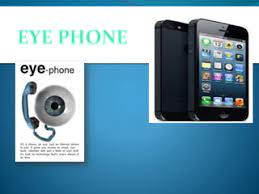
\includegraphics[width=.70\linewidth]{eyephone1.jpg}
\end{figure}

\chapter{Features and Specifications}

The Eyephone is renowned for its cutting-edge features and specifications, offering users a powerful and versatile mobile experience. With each new generation, the Eyephone introduces enhancements and advancements that push the boundaries of smartphone technology. Here are some of the notable features and specifications of the Eyephone:

\section{Display} 
The Eyephone boasts a stunning and vibrant display, featuring high resolution and color accuracy. With advanced OLED or Retina displays, users can enjoy crisp and detailed visuals, making it ideal for multimedia consumption, gaming, and productivity tasks.
\section{Camera System}
The Eyephone's camera system is renowned for its exceptional image quality and versatility. With advanced image sensors, optical image stabilization, and computational photography features, users can capture stunning photos and videos even in challenging lighting conditions. The Eyephone also offers a range of photography modes and editing tools to enhance creativity.
\section{Operating System}
The Eyephone runs on a sophisticated and user-friendly operating system, which provides a seamless and intuitive user experience. With regular updates and new features, the operating system ensures optimal performance, enhanced security, and access to a vast ecosystem of applications.
\section{Biometric Security}
The Eyephone incorporates advanced biometric security features, such as Face ID or Touch ID, to ensure secure and convenient device unlocking and authentication. These technologies use facial recognition or fingerprint scanning to provide a seamless and reliable security solution.
\section{Battery Life}
The Eyephone is equipped with high-capacity batteries that provide extended usage time. With efficient power management features, users can enjoy prolonged battery life, enabling them to stay connected and productive throughout the day.

\chapter{Applications}

\section{Health and Fitness}
Eyephone applications cater to health and fitness enthusiasts, offering features for tracking workouts, monitoring health metrics, and promoting a healthy lifestyle. Apps like Apple Health, Fitness, and various third-party fitness apps provide features like step counting, calorie tracking, heart rate monitoring, guided workouts, and sleep tracking.

\begin{figure}[h]
	\centering
	\hspace{21pt}
	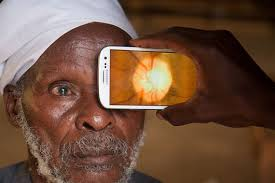
\includegraphics[width=.70\linewidth]{eyephone2.jpg}
\end{figure}

\section{Communication and Social Networking}
The Eyephone provides various applications for communication, including messaging apps, video calls, and social networking platforms. Users can stay connected with friends, family, and colleagues through apps like iMessage, WhatsApp, FaceTime, Facebook, Instagram, and Twitter.
	
\section{Productivity and Organization}
The Eyephone offers a wide range of productivity applications to help users stay organized, manage tasks, and enhance their work efficiency. Applications like Notes, Calendar, Reminders, and Email clients allow users to create, organize, and synchronize their schedules, to-do lists, and important information.

\section{Multimedia and Entertainment}
With its advanced display and powerful hardware, the Eyephone is an excellent platform for multimedia consumption and entertainment. Users can enjoy streaming services like Apple Music, Spotify, Netflix, and YouTube, as well as access a vast collection of games, e-books, podcasts, and digital magazines.

\section{Finance and Banking}
Many banking institutions provide applications for Eyephone users to manage their finances conveniently. These apps allow users to check account balances, transfer funds, pay bills, and monitor transactions securely.

\chapter{Challenges}

\section{Storage Limitations}
Eyephones come with different storage options, but even the highest capacity models may face limitations when users accumulate large amounts of data, including photos, videos, and applications. Managing and optimizing storage space can be a challenge, especially for users who heavily rely on their devices for multimedia content.

\section{Cost}
Eyephones are considered premium devices with a higher price point compared to other smartphones. Affordability can be a challenge for some users, especially in regions where the cost of the device may pose a barrier to ownership. Additionally, repairs and replacements can also be costly, making it important for users to consider budgetary constraints.

\section{Software Compatibility}
With the release of new Eyephone models and operating system updates, some older applications or features may become incompatible or experience compatibility issues. Users may face challenges in finding updated versions or alternative applications that work seamlessly with their device's software.

\section{Learning Curve}
For users who are new to Eyephones or transitioning from other operating systems, there can be a learning curve in familiarizing themselves with the device's interface, features, and gestures. Getting accustomed to the device and optimizing its functionality may take some time and effort.

\section{Fragmented Ecosystem}
While Eyephones offer a seamless integration with Apple's ecosystem, including Mac computers, iPads, and other Apple devices, there can be challenges when attempting to integrate or sync with non-Apple devices or services. Interoperability with different platforms and ecosystems may require additional steps or workarounds.

\chapter{Future of Eyephone}
The future of Eyephone holds exciting possibilities as technology continues to advance and consumer demands evolve. Here are some potential aspects that could shape the future of Eyephones:

\section{Enhanced Augmented Reality (AR) Experiences}
 Eyephones are already equipped with AR capabilities, but the future may bring even more immersive and advanced AR experiences. This could include improved AR applications for gaming, education, navigation, and more, blurring the lines between the digital and physical worlds.
 
 \begin{figure}[h]
	\centering
	\hspace{21pt}
	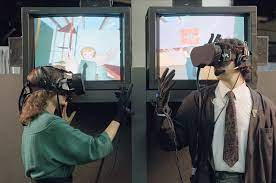
\includegraphics[width=.70\linewidth]{eyephone0.jpg}
\end{figure}

\section{Foldable and Flexible Displays}
The introduction of foldable and flexible display technology opens up new avenues for Eyephones. Foldable devices offer the convenience of a larger screen when needed while maintaining portability. As this technology evolves, we may see Eyephones with foldable or flexible displays that provide users with enhanced multitasking and creative possibilities.

\section{Advanced Biometric Features}
Eyephones have already incorporated biometric authentication with Face ID, but future iterations may introduce even more advanced biometric features. This could include under-display fingerprint sensors, iris scanning, or even new forms of biometric identification that enhance security and user convenience.

\section{Integration with Internet of Things}
The Internet of Things is expanding rapidly, and Eyephones are expected to seamlessly integrate with smart home devices, wearables, and other IoT devices. This integration would enable users to control and monitor their connected devices directly from their Eyephones, enhancing convenience and connectivity.

\chapter{Conclusion}
In conclusion, synchronous chip design plays a crucial role in the development of digital systems, enabling precise timing control, coordinated operations, and reliable data processing. It has evolved significantly with the introduction of various techniques and advances to address key challenges and optimize performance.

Recent developments in synchronous chip design have focused on areas such as power optimization, clock gating, high-speed designs, and adaptive power management. Techniques like clock gating and voltage scaling help reduce power consumption, while high-speed designs and advanced interconnects enable higher data transfer rates and improved signal integrity. Additionally, design methodologies for low-power design, timing closure, and design for manufacturability have advanced, resulting in more energy-efficient and reliable chips.

These advancements reflect the industry's efforts to meet the growing demands for higher performance, lower power consumption, and improved chip functionality. As technology continues to progress, synchronous chip design will continue to evolve, leveraging new techniques and methodologies to address future challenges and push the boundaries of digital system design.

Overall, synchronous chip design remains a critical discipline in the development of various applications, including microprocessors, digital signal processing, networking systems, and embedded systems. The advancements in synchronous chip design contribute to the development of more efficient, reliable, and high-performance digital systems that power our modern world.

\chapter{References}

\begin{itemize}
\item[[1]] EyePhone: activating mobile phones with your eyes

https://dl.acm.org/doi/abs/10.1145/1851322.1851328

\item[[2]] The Eyephone: a head-mounted stereo display

https://www.spiedigitallibrary.org/conference-proceedings-of-spie/1256/0000/The-Eyephone-a-head-mounted-stereo-display/10.1117/12.19902.short?SSO=1

\item[[3]] The Eye Phone Study: reliability and accuracy of assessing Snellen visual acuity using smartphone technology

https://www.nature.com/articles/eye201560

\vspace{12pt}
\end{itemize}
\end{document}
